\section{}
Watch the BBQ Temperature Control video posted on eClass.
\subsection{}
\textit{What are the reference signal and plant output for this system?} 

For this system, the reference signal is the desired temperature of the BBQ, and the plant output is the actual temperature of the BBQ.

\subsection{}
\textit{What is a disturbance for this system?}

For this system, a disturbance are environmental factors that affect the temperature of the BBQ, such as wind, rain, ambient temperature, etc.

\subsection{}
\textit{Draw a block diagram of the overall closed-loop system. Label the signal arrows and name
the controller, actuator, plant and sensor in your diagram.}

\begin{figure}[h]
    \centering
    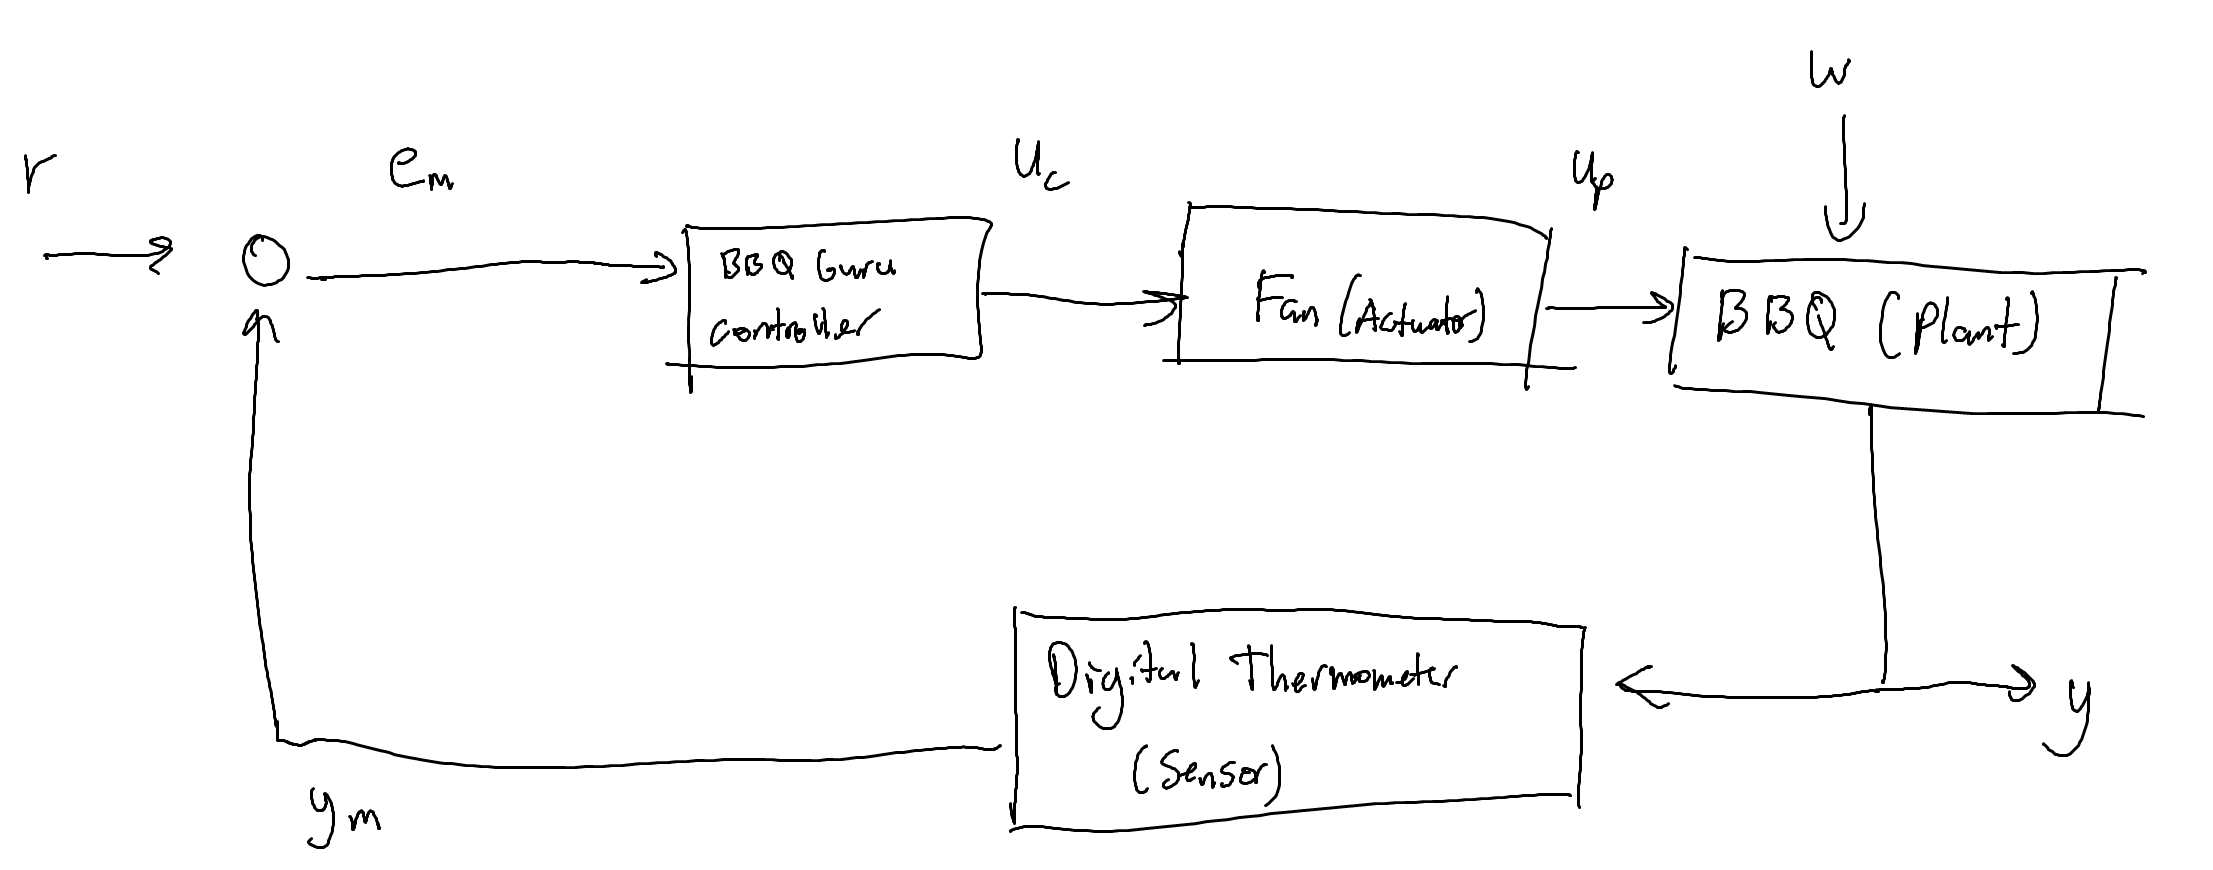
\includegraphics[width=0.8\textwidth]{Questions/Figures/Q1c.png}
    \caption{Block diagram of the overall closed-loop system for BBQ Guru.}
    \label{fig:Q1c}
\end{figure}

Where
\begin{itemize}
    \item $r$ is the reference signal, the desired temperature of the BBQ
    \item $e_m$ is the measured tracking error, the difference between the desired temperature and the measured temperature of the BBQ
    \item $u_c$ is the control input, which is the output of the controller to the fan 
    \item $u_p$ is the plant input, which is the fan speed which controls the amount of oxygen supplied to the charcoal, affecting the temperature of the BBQ
    \item $y$ is the plant output, the actual temperature of the BBQ
    \item $y_m$ is the measured plant output, the measured temperature of the BBQ from the temperature sensor as an electronic signal
    \item $w$ is the disturbance, which is the environmental factors that affect the temperature of the BBQ
    \item $v$ is the sensor noise, which is the noise from the temperature sensor
\end{itemize}
